\section{Training operators to assemble a starter engine}\label{sec:results}

Results text.

\subsection{Testing platforms}

\begin{itemize}
	\item BenQ W1070 FHD DLP projector
	\item Asus Xtion Pro Live structured light 3d sensor
	\item Kinect 2 Time Of Flight (ToF) 3D sensor
	\item David Laser Structure Light System
\end{itemize}

\begin{figure}[ht]
	\centering
	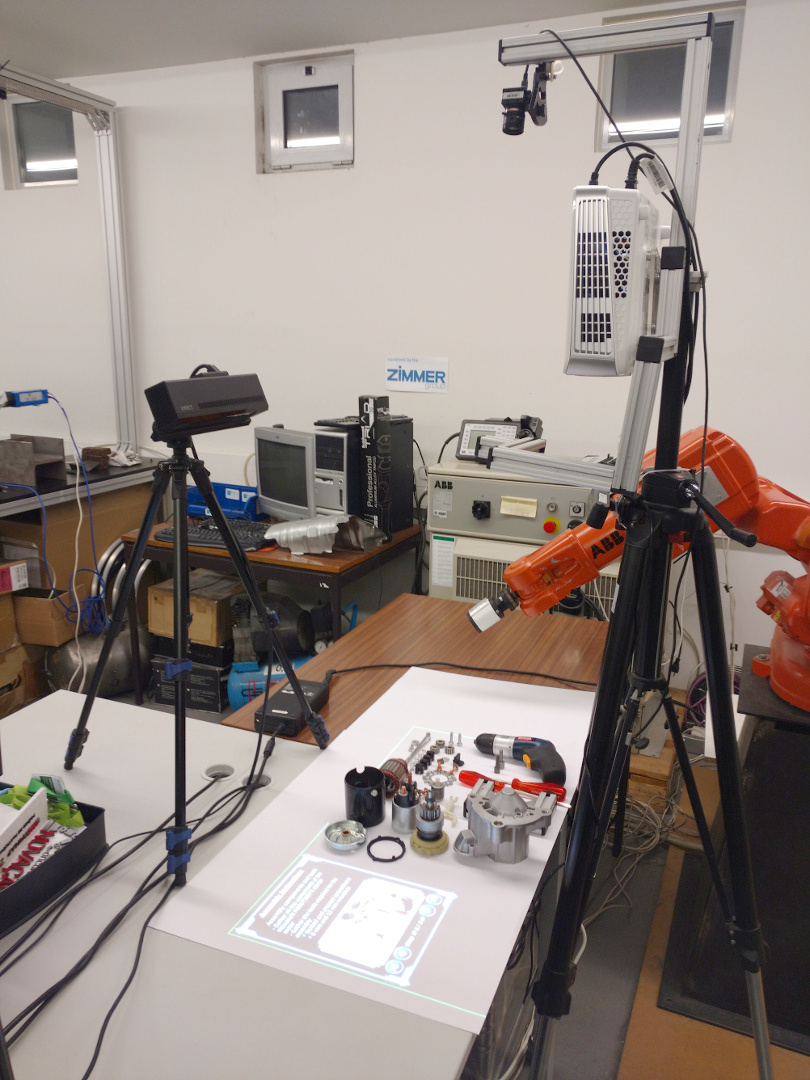
\includegraphics[width=0.4\linewidth]{hardware}
	\caption{Hardware setup}
	\label{fig:hardware}
\end{figure}


\subsection{Training session}

\begin{figure}[H]
	\begin{floatrow}[2]
		\ffigbox[\FBwidth]
		{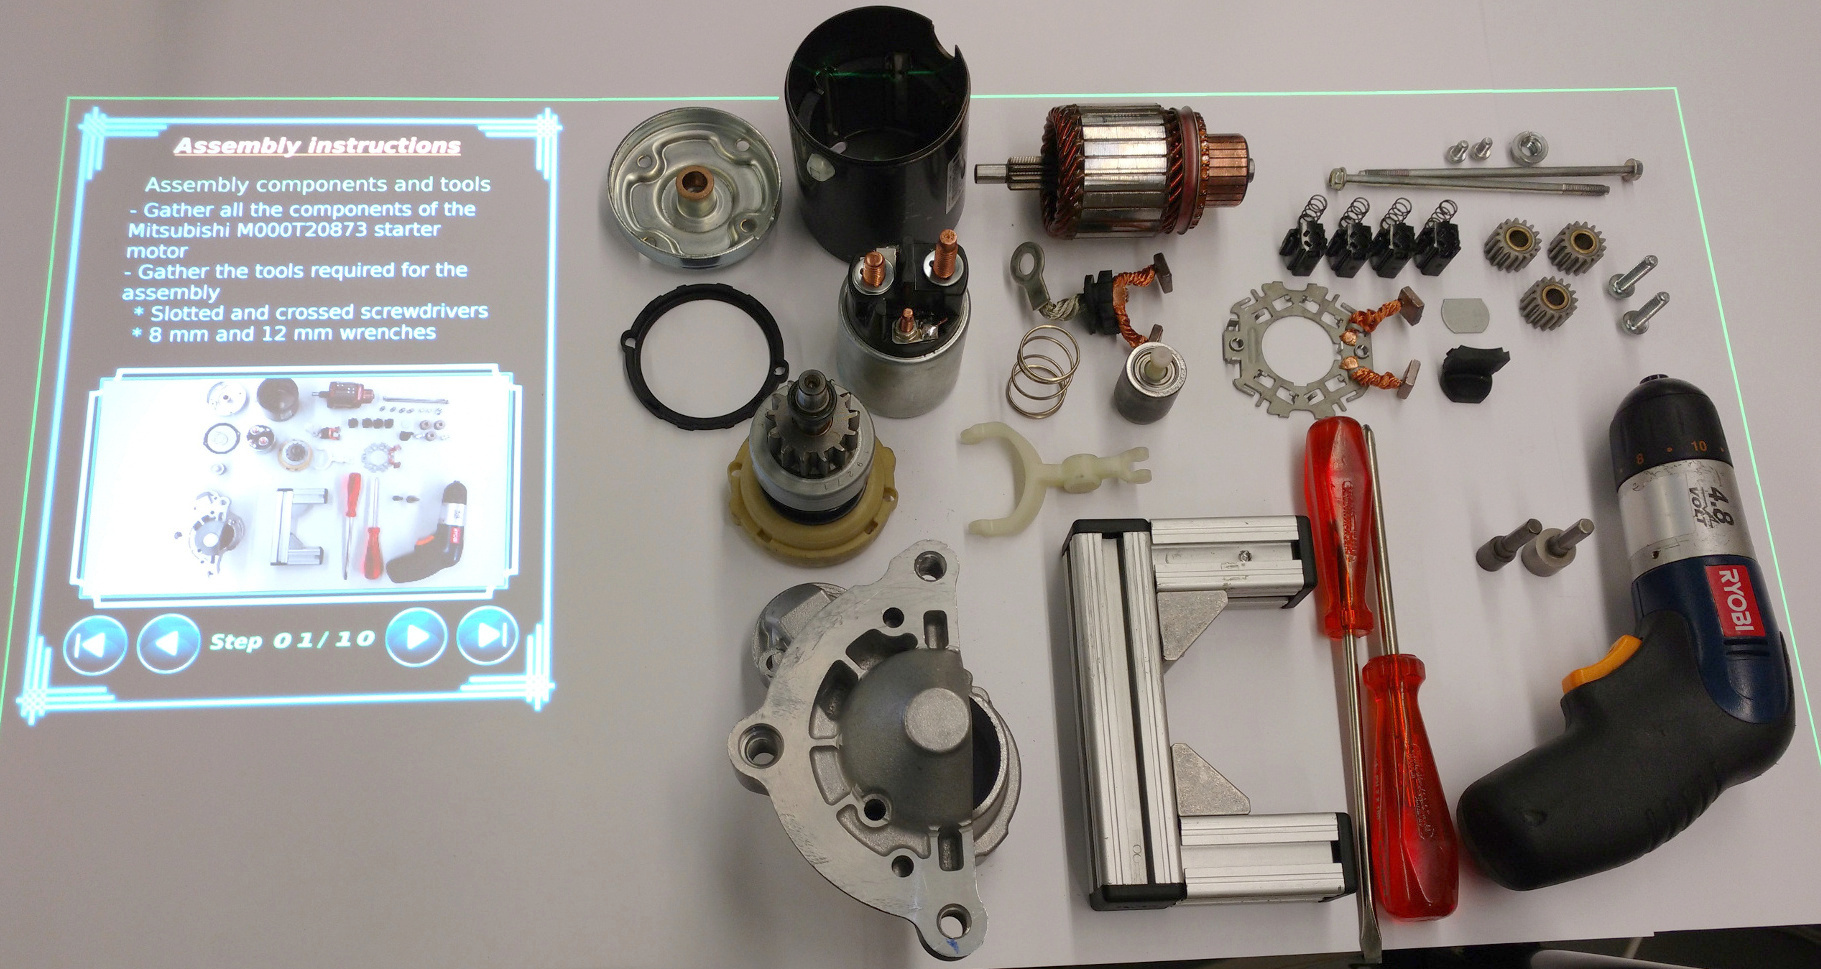
\includegraphics[height=.164\textheight]{assembly-parts}}
		{\caption{Assembly parts}\label{fig:assembly-parts}}
		\ffigbox[\FBwidth]
		{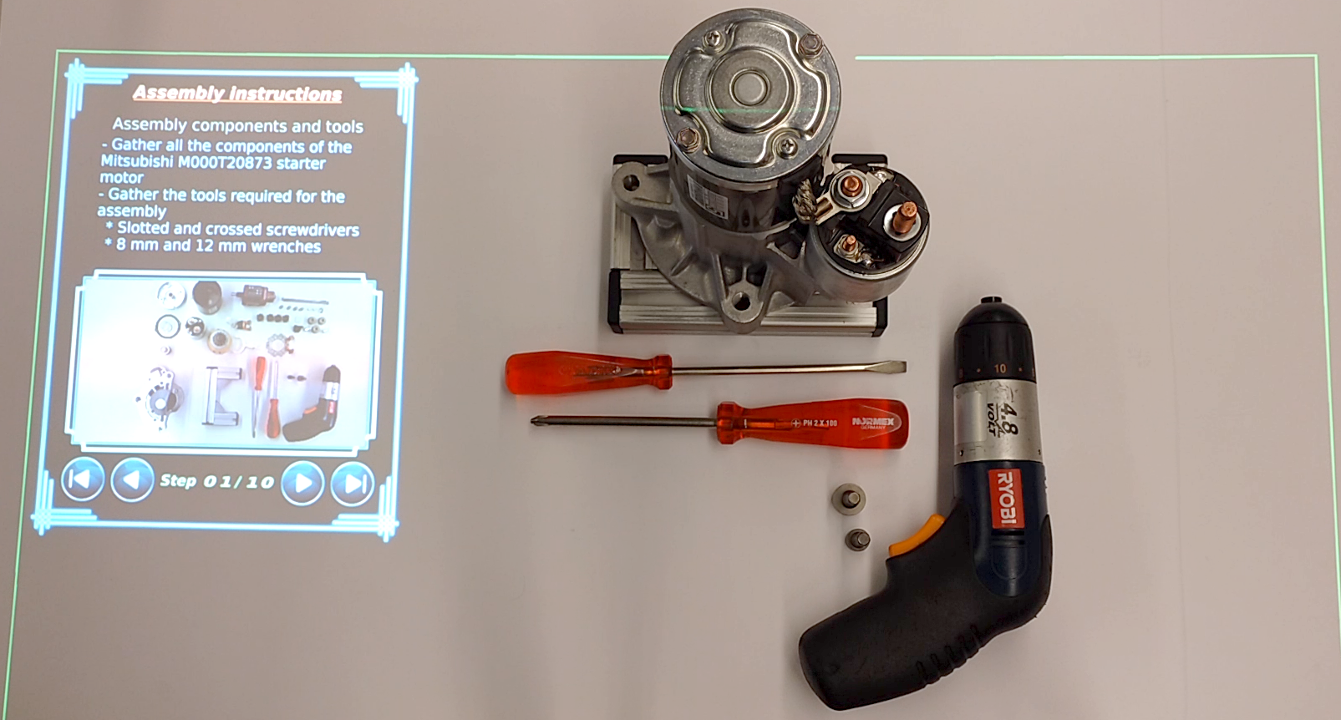
\includegraphics[height=.164\textheight]{assembled-object}}
		{\caption{Assembled object}\label{fig:assembled-object}}
	\end{floatrow}
\end{figure}

\begin{figure}[H]
	\begin{floatrow}[2]
		\ffigbox[\FBwidth]
		{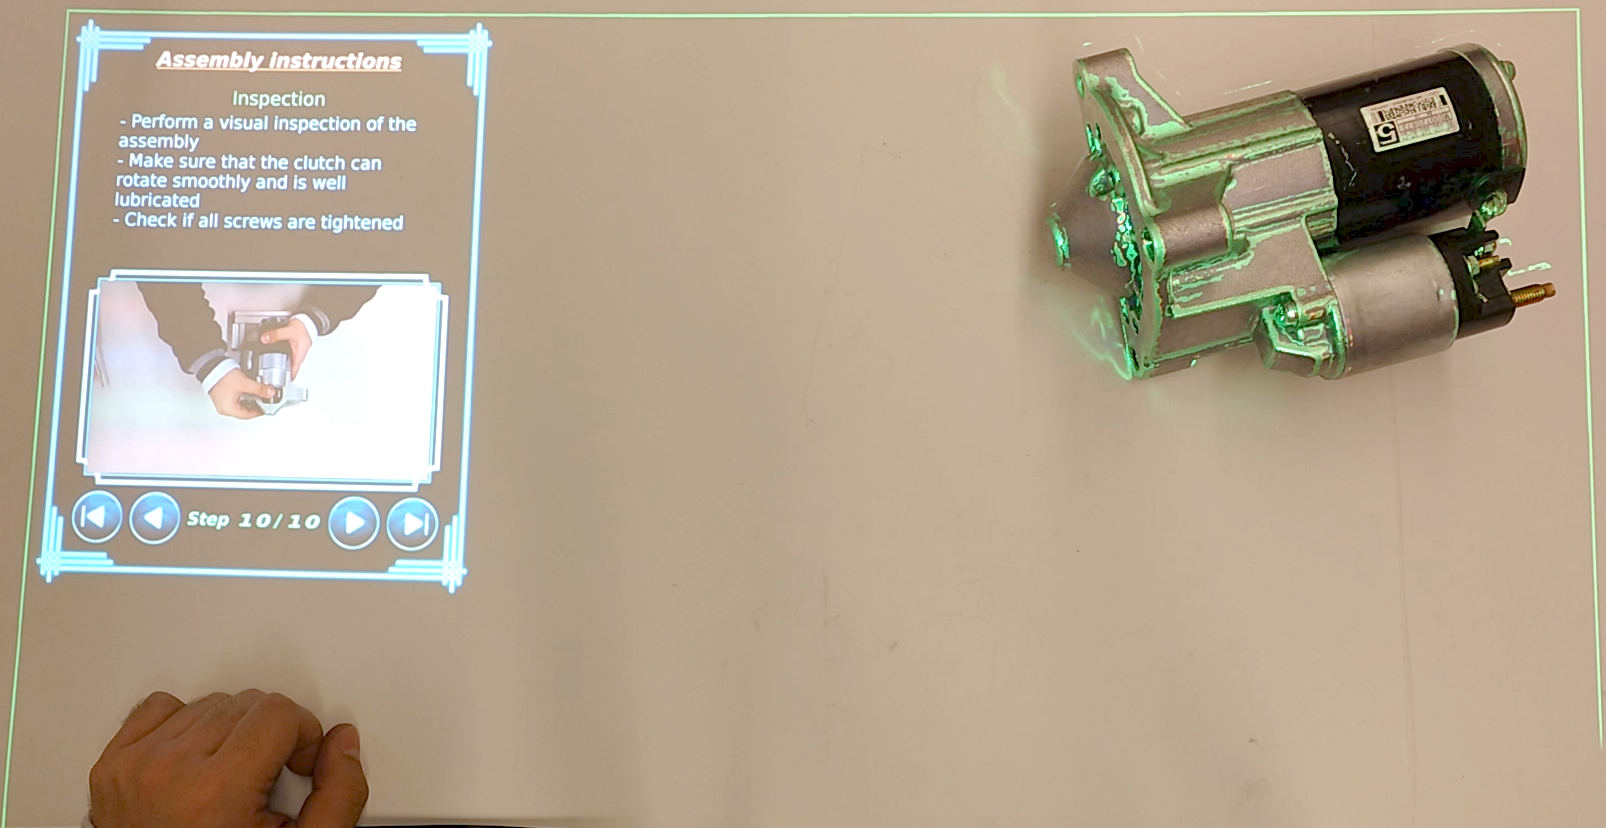
\includegraphics[height=.165\textheight]{projection-mapping-1}}
		{\caption{Projection of the reconstructed 3D model (texture colorized by surface normal curvature in Meshlab)}\label{fig:projection-mapping-1}}
		\ffigbox[\FBwidth]
		{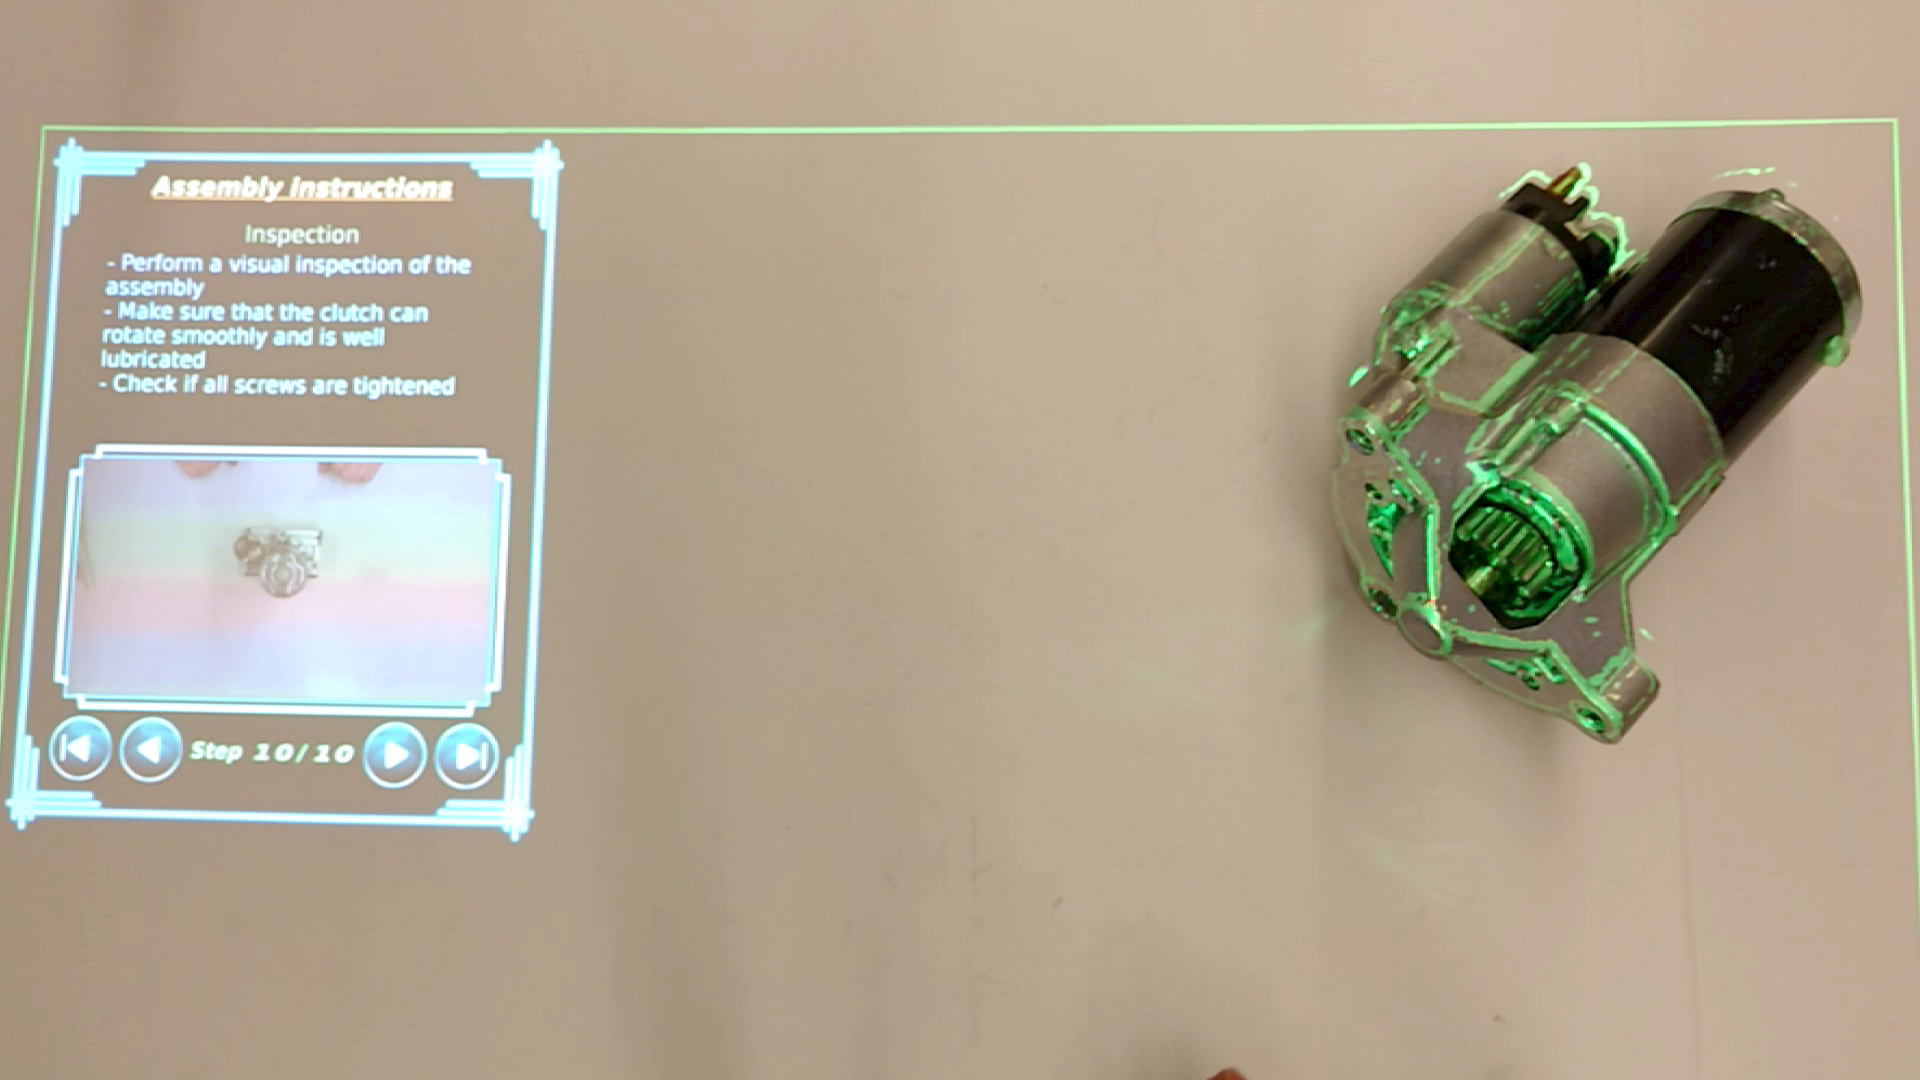
\includegraphics[height=.165\textheight]{projection-mapping-2}}
		{\caption{Detailed view of the assembled object projection}\label{fig:projection-mapping-2}}
	\end{floatrow}
\end{figure}



\begin{figure}[H]
	\begin{floatrow}[4]
		\ffigbox[\FBwidth]
		{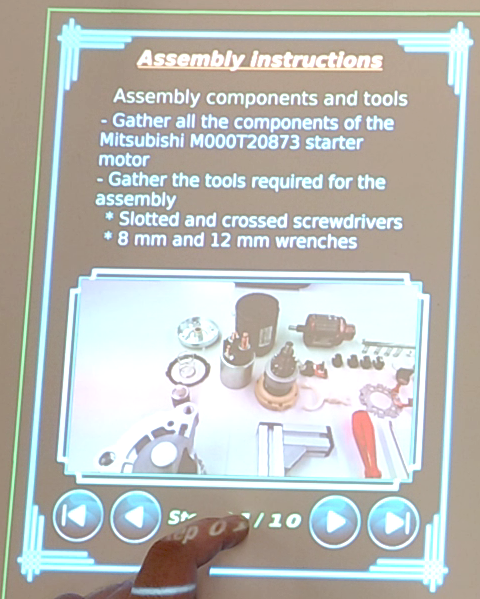
\includegraphics[height=.177\textheight]{interaction-pause}}
		{\caption{Example of video pause / play interaction}\label{fig:interaction-pause}}
		\ffigbox[\FBwidth]
		{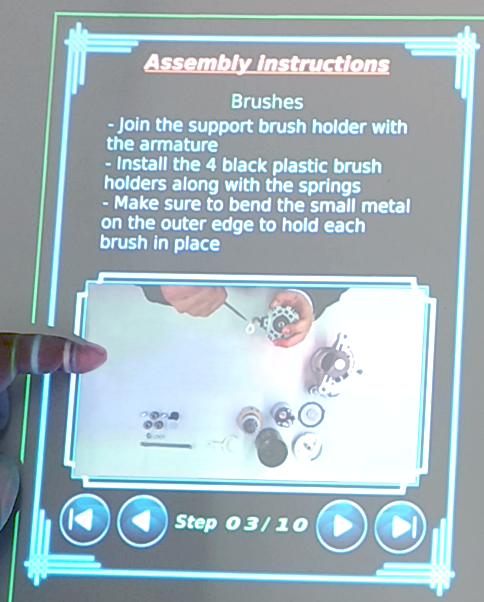
\includegraphics[height=.177\textheight]{interaction-seek}}
		{\caption{Example of video seek interaction}\label{fig:interaction-seek}}
		\ffigbox[\FBwidth]
		{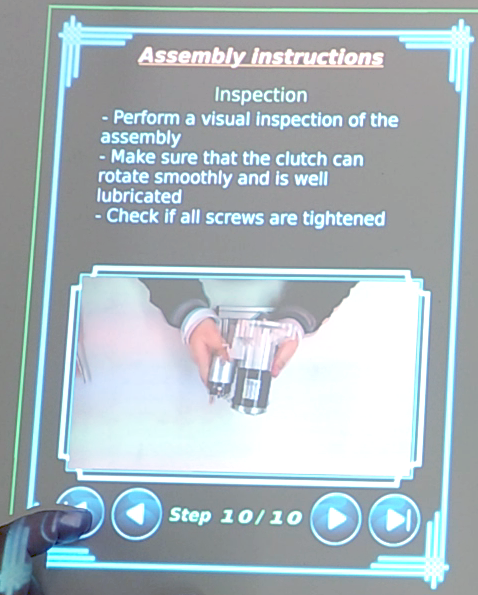
\includegraphics[height=.177\textheight]{interaction-first-0}}
		{\caption{Example of request to move to first assembly step}\label{fig:interaction-first-0}}
		\ffigbox[\FBwidth]
		{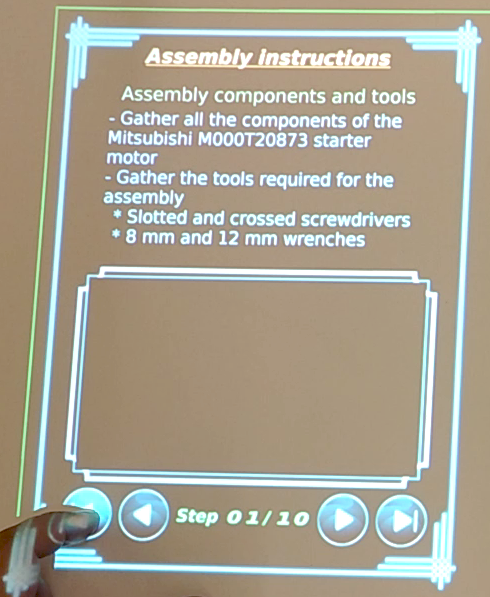
\includegraphics[height=.177\textheight]{interaction-first-1}}
		{\caption{Visual feedback that the request to move to the first assembly step was recognized}\label{fig:interaction-first-1}}
	\end{floatrow}
\end{figure}


%\begin{figure}[H]
%	\begin{floatrow}[2]
%		\ffigbox[\FBwidth]
%		{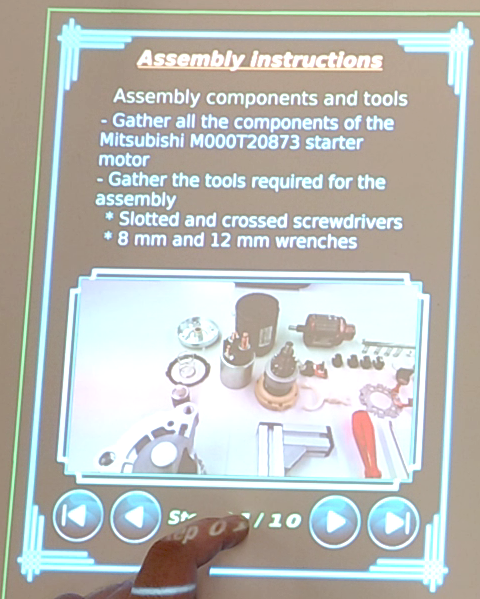
\includegraphics[height=.3\textheight]{interaction-pause}}
%		{\caption{Example of video pause / play interaction}\label{fig:interaction-pause}}
%		\ffigbox[\FBwidth]
%		{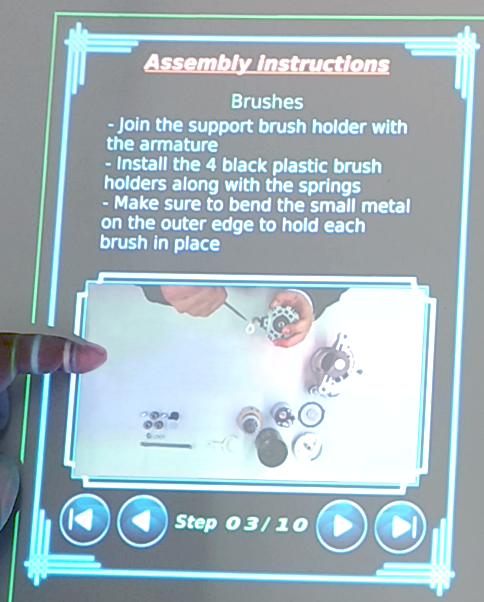
\includegraphics[height=.3\textheight]{interaction-seek}}
%		{\caption{Example of video seek interaction}\label{fig:interaction-seek}}
%	\end{floatrow}
%\end{figure}
%
%\begin{figure}[H]
%	\begin{floatrow}[2]
%		\ffigbox[\FBwidth]
%		{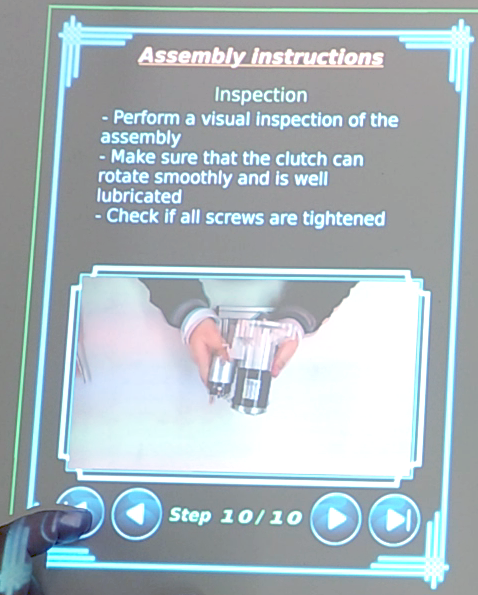
\includegraphics[height=.3\textheight]{interaction-first-0}}
%		{\caption{Example of request to move to first assembly step}\label{fig:interaction-first-0}}
%		\ffigbox[\FBwidth]
%		{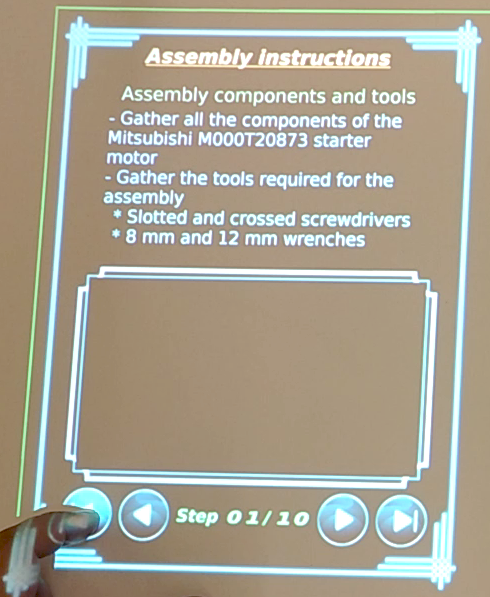
\includegraphics[height=.3\textheight]{interaction-first-1}}
%		{\caption{Visual feedback that the request to move to the first assembly step was recognized}\label{fig:interaction-first-1}}
%	\end{floatrow}
%\end{figure}
